\documentclass[11pt]{article}
\usepackage[doi=false,isbn=false,maxcitenames=10,maxbibnames=10,abbreviate=false,style=alphabetic]{biblatex}
\addbibresource{cv.bib}

\newtoggle{usecoe}
\settoggle{usecoe}{false}
\newcommand{\coe}[1]{\iftoggle{usecoe}{#1}{}}
\newcommand{\notcoe}[1]{\nottoggle{usecoe}{#1}{}}
\newcommand{\coeite}[2]{\iftoggle{usecoe}{#1}{#2}}

\usepackage[T1]{fontenc}
\usepackage{enumitem}
\usepackage{amsmath}
\usepackage{amssymb}
\notcoe{
  \usepackage{graphicx}
  \usepackage{wrapfig}
}
\usepackage{complexity}
\usepackage{booktabs}
\usepackage{hyperref}
\hypersetup{
  colorlinks=true, %set true if you want colored links
  linkcolor=blue,
  filecolor=blue,  
  linktoc=all,     %set to all if you want both sections and subsections linked
  linktocpage=true,
}

\setitemize{noitemsep,topsep=0pt,parsep=0pt,partopsep=0pt}
\usepackage[margin=0.8in]{geometry}

\newcommand{\myname}{ThanhVu Huy Nguyen}
\newcommand{\mynamevn}{Nguy$\tilde{\hat{\text{e}}}$n Huy ThanhV$\tilde{\text{u}}$}
\newcommand{\myemail}{nguyenthanhvuh@gmail.com}
\newcommand{\myemailwork}{tvn@gmu.edu}
\newcommand{\myweb}{https://nguyenthanhvuh.github.io}
\newcommand{\mygooglescholar}{\href{https://scholar.google.com/citations?user=TLcVQ-MAAAAJ}{Google Scholar}}
\newcommand{\emailweb}{
\item Email: \href{mailto:\myemailwork}{\myemailwork}
\item Web: \url{\myweb}
}

\newcommand{\mypubcc}[1]{\item~\label{#1} \fullcite{\detokenize{#1}c}}
\newcommand{\mypubc}[2]{\item~\label{#1} \fullcite{#1c}\coe{, contribution #2}}   %label,contribution percentage (optional)

\begin{document}
\thispagestyle{empty}

\begin{center}
  \textbf{\Huge {\myname}: \\
    Curriculum Vitae}
\end{center}

\tableofcontents
\newpage
\setcounter{page}{1}

\coeite{
  \setcounter{section}{-1}
  \section{Version}  
  \begin{itemize}
  \item Candidate Name: \myname{}
  \item Candidate Title: Assistant Professor
  \item Unit Name: Department of Computer Science and Engineering
  \item Office Address: 364 Avery Hall, University of Nebraska-Lincoln, Lincoln, NE 68523
    \emailweb{}
  \end{itemize}
  
  \begin{table}[htbp]
    \caption{Table of Changes Made to CV since Original Submission}
    \small
    \centering
    \begin{tabular}{ccl}
      \toprule
      Version & Date & Changes (listed by subsection \#)\\
      \midrule
      1 & 1/30/2020 & Original version\\
      2 & 1/28/2021 & Version 2: change to \LaTeX\ format\\
      \bottomrule
    \end{tabular}
  \end{table}
}
{
  \section{Personal}

  \begin{minipage}{.8\textwidth}
    \begin{itemize}
    \item Name: \myname{}
      \begin{description}
      \item In Vietnamese: \mynamevn{}
      \end{description}
    \item Contact Info:
      \begin{itemize}
        \item Nguyen Engineering Building 4430, 4400 University Drive, Fairfax, VA 22030
        \emailweb{}
      \end{itemize}
    \item Citizenship: U.S
      \begin{itemize}
      \item DoD Secret Clearance (inactive)
      \end{itemize}
    \end{itemize}
  \end{minipage}
  \begin{minipage}{.3\textwidth}
    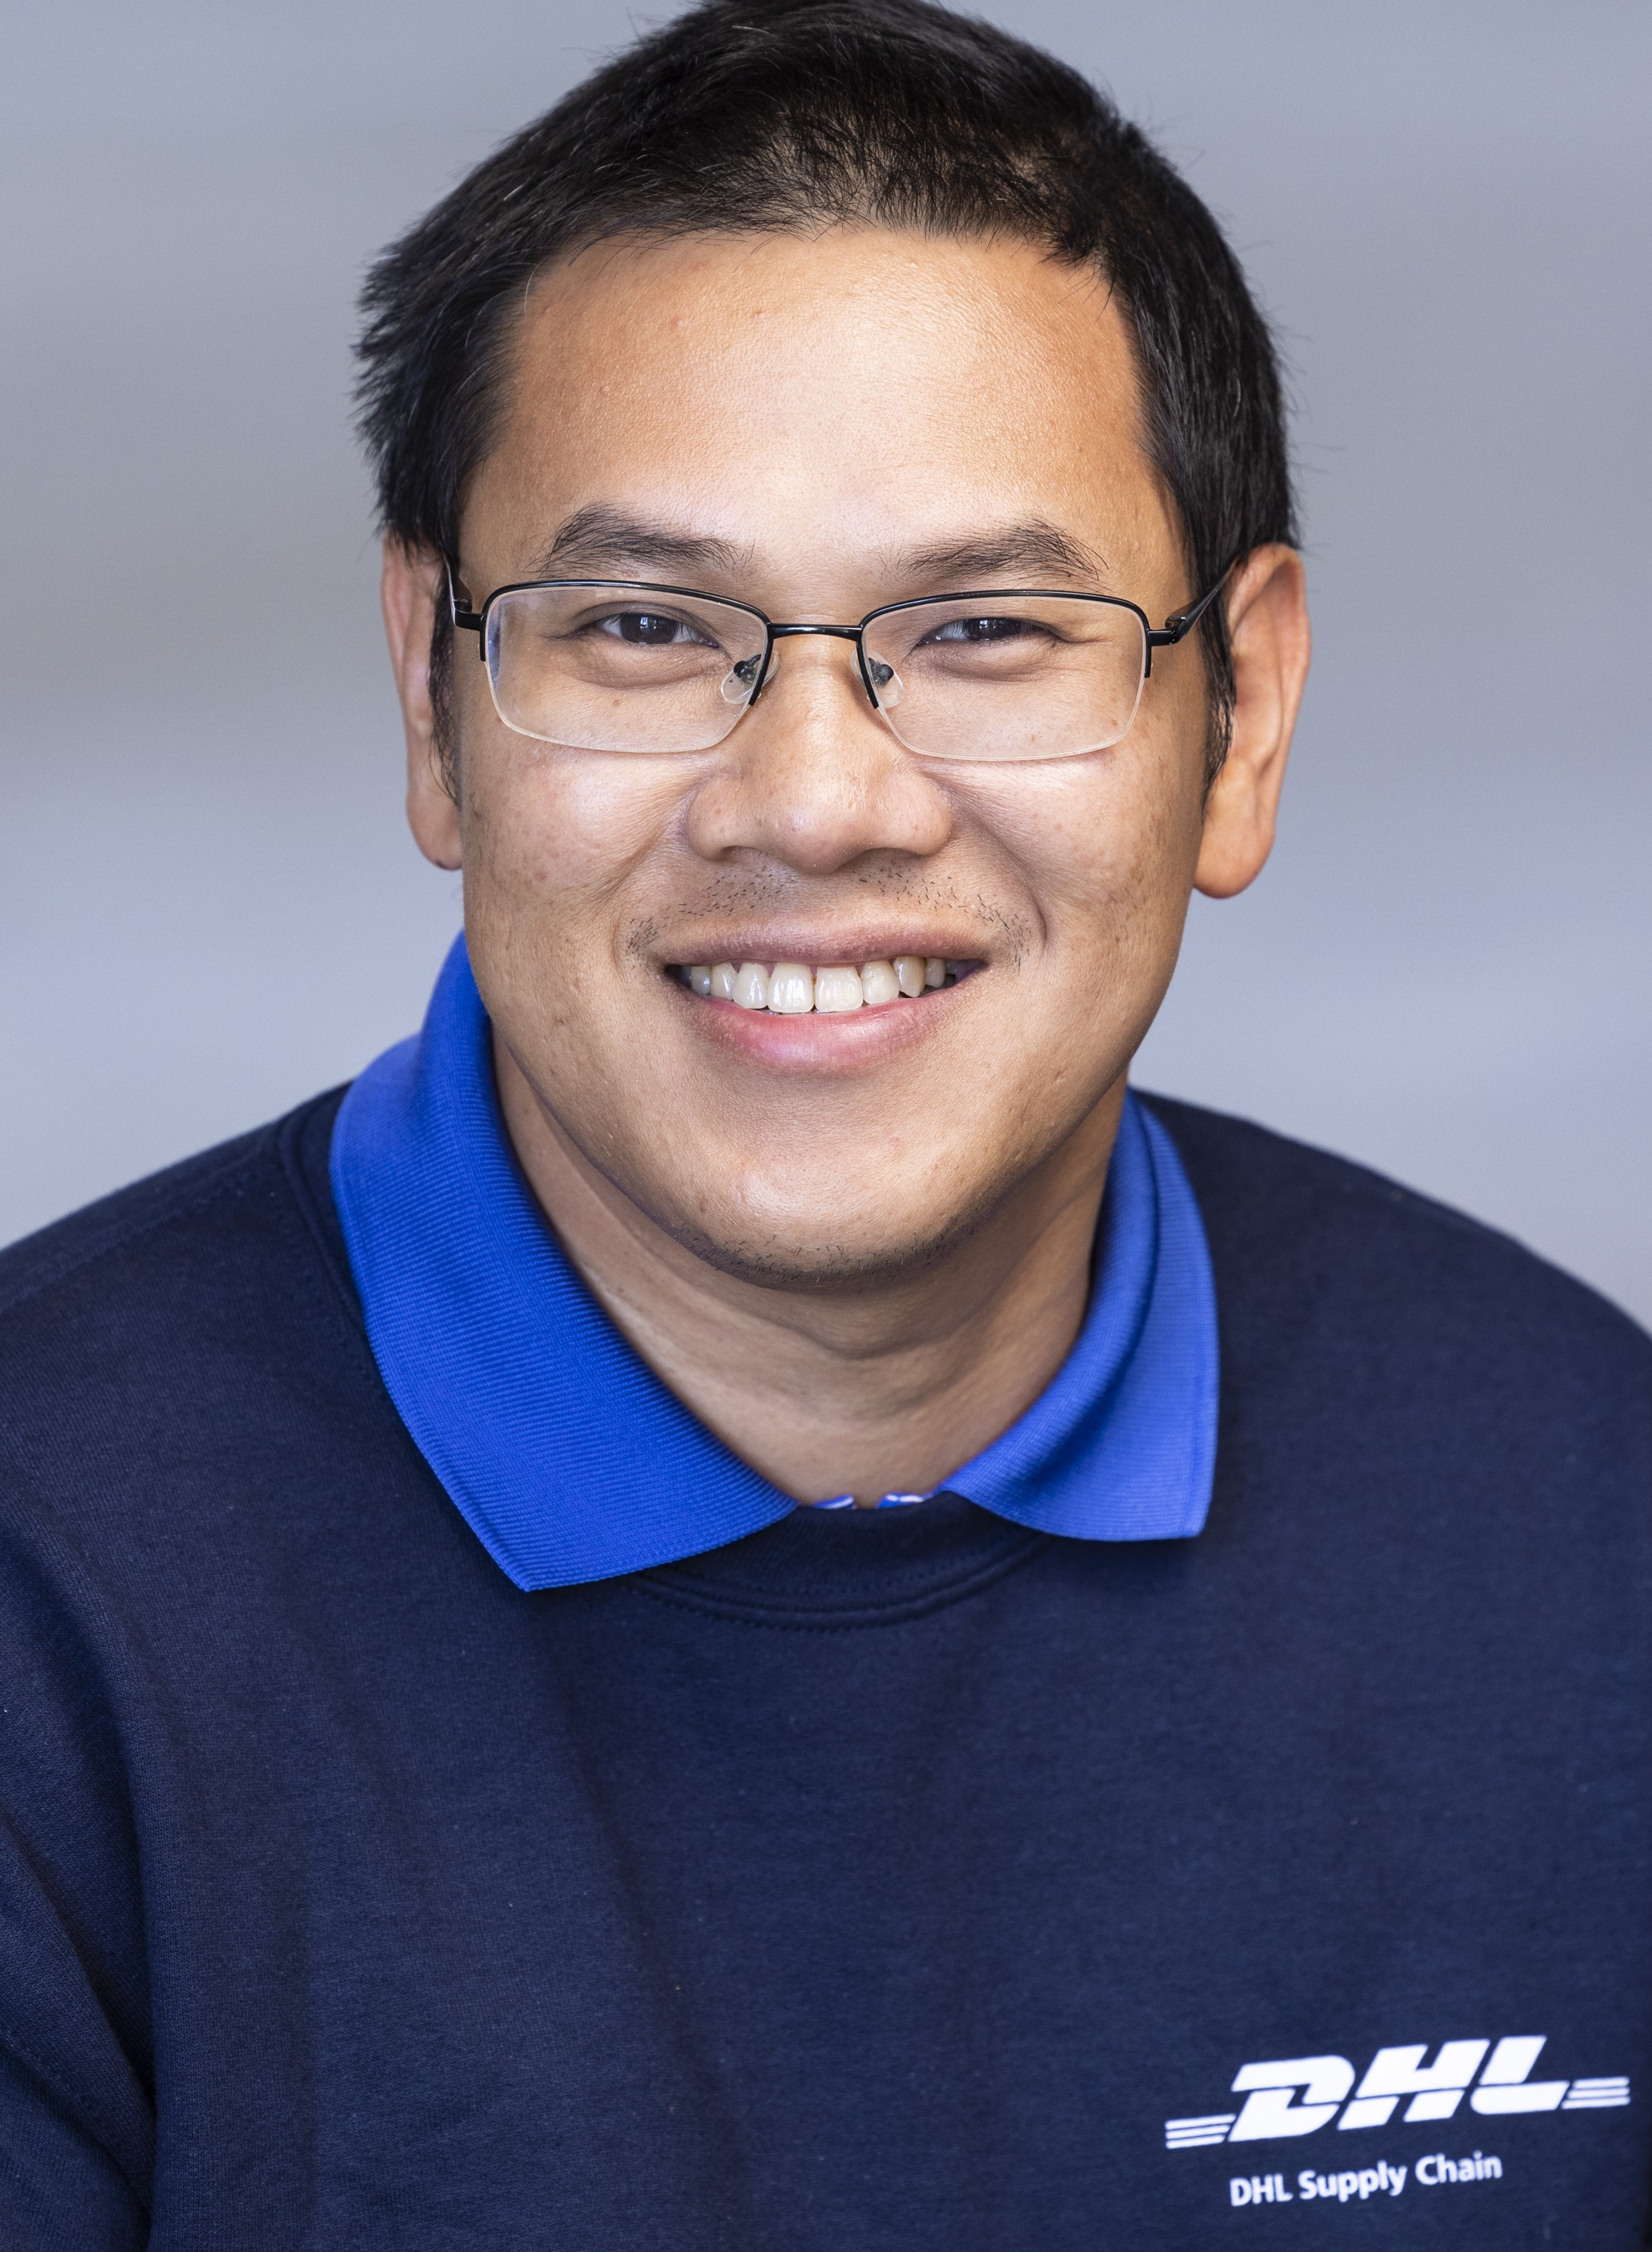
\includegraphics[width=0.4\textwidth]{tvn.png}
  \end{minipage}

  \paragraph{Bio.} ThanhVu Nguyen is an assistant professor in the Department of Computer Science at George Mason University. 
  Prior to joining GMU, he was at the University of Nebraska-Lincoln. He received his Ph.D. in Computer Science from the University of New Mexico-Albuquerque and completed a two-year postdoc at the University of Maryland-College Park.

  His research is in the intersection of Software Engineering and Programming Languages. In particular, he focuses on improving software quality through dynamic invariant inference,  automatic program repair, and highly-configurable systems analysis.
He is a recipient of the NSF CISE Career Research Initiation Initiative (CRII) Award, a 10-year Most Influential Paper award (at ICSE 2019), and a 10-year Most Impact Paper Award (at GECCO 2019).
}

\section{Education and Employment History}

\subsection{Education}

\begin{itemize}
\item \textbf{Postdoc}, Computer Science,  \href{https://www.umd.edu}{University of Maryland}, College Park, MD\hfill 2014--2016
  \begin{description}
  \item Mentor: Jeff Foster
  \item Research Topic: Analyzing Highly-Configurable Systems and Invariant Generation
  \end{description}
  
\item \textbf{Ph.D.}, Computer Science,  \href{https://www.unm.edu}{University of New Mexico}, Albuquerque, NM\hfill 2007--2014
  \begin{description}
  \item Advisers: Stephanie Forrest and Deepak Kapur
  \item Dissertation: Automatic Program Repair and Dynamic Invariant Generation~[\ref{nguyen2014automating}]
  \end{description}

\item \textbf{M.S.}, Computer Science,  \href{https://www.hbg.psu.edu}{Penn State University}, Harrisburg, PA\hfill 2003--2006
  \begin{description}
  \item Adviser: Thang N. Bui
  \item Thesis: Using Ant-based Algorithms to solve \NP-Complete graph problems~[\ref{nguyen2006graph}]
  \end{description}
  
\item \textbf{B.S.}, Computer Science, \href{https://www.psu.edu}{Penn State University}, University Park, PA \hfill 1999--2003
  \vspace{0.1in}
\item \textbf{High School}
  \begin{itemize}
  \item \href{https://www.bishopmcdevitt.org/mcd/}{Bishop McDevitt}, Harrisburg, PA \hfill 1997--1999
  \item \href{https://www.mckinley.k12.hi.us/}{McKinley High School}, Honolulu, HI \hfill 1995--1997  
\end{itemize}
\end{itemize}


\subsection{Employment History}

\begin{itemize}
\item Assistant Professor, Department of Computer Science, \href{https://cs.gmu.edu}{George Mason University}\hfill 2021--current  
\item Assistant Professor, School of Computing, \href{https://computing.unl.edu}{University of Nebraska-Lincoln}\hfill 2016--2021
\item Postdoc, Department of Computer Science, \href{https://www.cs.umd.edu}{University of Maryland-College Park}\hfill 2014--2016
\item Research Assistant, Dept. of Computer Science, \href{https://www.cs.unm.edu}{University of New Mexico-Albuquerque}\hfill 2007--2014
\item Internship, Information Technology Division, \href{https://www.nrl.navy.mil}{Naval Research Laboratory}\hfill 2012--2013
\item Internship, Advanced Technology Laboratories, \href{https://lockheedmartin.com/en-us/capabilities/research-labs/advanced-technology-labs.html}{Lockheed Martin}\hfill 2007
\item Internship, Tactical Electrical Warfare Division,  \href{https://www.nrl.navy.mil}{Naval Research Laboratory}\hfill 2004--2016
\end{itemize}

\coe{
  \subsection{Apportionment at UNL}
  \begin{itemize}
  \item Research: 45\%, Teaching: 45\%, Service: 10\%
  \end{itemize}
}
\section{Research \coe{Accomplishments}}

\notcoe{
  \subsection{Research Interests}
  Software Engineering; Programming Languages; Software Testing, Verification, and Analysis; Software Correctness and Reliability; Dynamic Invariant Generation; Automatic Program Repair.  
}

\subsection{Publication Record}

\paragraph{Notes:}
\begin{itemize}
\item \(^1\), \(^2\), \(^3\) denote co-authorship with my undergraduate, M.S., and Ph.D. students, respectively.
\item  \textbf{Bold journal and conference names} indicate full research papers at top-tier venues (e.g., TSE, OOPSLA, ICSE, FSE, PLDI). See \href{https://csrankings.org}{csrankings.org} for top CS conferences.
\item In computer science, full research conference papers are full-length and rigorously reviewed by at least three peers. Top-tier conferences have acceptance rates comparable to or even lower than leading journals.
\item Citations (\mygooglescholar{}): 3228, h-index 15, i10-index 22 (as of Oct'22).  
\end{itemize}

\emergencystretch=1em
\newcommand{\mybooks}{
  \begin{enumerate}
    \mypubcc{kapur2013geometric}
  \end{enumerate}
}

\newcommand{\myjournals}{
  \begin{enumerate}[label=J\arabic*]
    
    \mypubcc{nguyen2021using}
    \coe{\mypubcc{ishimwe2021dynaplex}}
    \coe{\mypubcc{le2020dynamite}}

    \coe{\mypubcc{mariano2019program}}

    \mypubcc{nguyen2014dig}

    \mypubcc{le2011genprog}
    \begin{itemize}
    \item \textbf{Featured Article}
    \item \textbf{1000+ citations}
    \end{itemize}
    
    \mypubcc{weimer2010automatic}
    \begin{itemize}
    \item \textbf{Research Highlight}
    \item \textbf{400+ citations}
    \end{itemize}
    
    \mypubcc{bui2008ant}
    \begin{itemize}
    \item \textbf{100+ citations}
    \end{itemize}
    
    \mypubcc{smith2007autonomous}
    
  \end{enumerate}
}

\newcommand{\myconfs}{
  \begin{enumerate}[label=C\arabic*]

    \mypubc{brida2022icebar}{14\%}
    \mypubc{zheng2022atr}{14\%}
    \mypubc{nguyen2022analyzing}{33\%}
    \mypubc{nguyen2022toward}{25\%}        
    \mypubc{ishimwe2022dynaplex}{33\%}    
    \mypubc{nguyen2022syminfer}{70\%}
    \notcoe{\mypubcc{ishimwe2021dynaplex}}    
    \mypubc{nguyen2021gentree}{50\%}
    \mypubc{zheng2021flack}{14\%}
    \mypubc{brida2021bounded}{14\%}
    \mypubc{nguyen2021tool}{50\%}
    \mypubc{zheng2021tool}{14\%}
    \mypubc{brida2021tool}{14\%}    

    \notcoe{\mypubcc{le2020dynamite}}
    \mypubc{nguyen2020using}{20\%}
    \mypubc{zheng2020debugging}{33\%}
    
    \mypubc{nguyen2020using2}{50\%}

    \mypubc{le2019sling}{33\%}
    
    \notcoe{\mypubcc{mariano2019program}}

    \mypubc{zheng2018automatic}{25\%}

    \mypubc{gazzillo2018localizing}{25\%}

    \mypubc{nguyen2017syminfer}{33\%}
    
    \mypubc{nguyen2017counterexample}{25\%}

    \mypubc{nguyen2017connecting}{33\%}

    \mypubc{nguyen2016igen}{20\%}

    \mypubc{nguyen2014using}{25\%}

    \mypubc{nguyen2012using}{25\%}
    \begin{itemize}
    \item \textbf{90+ citations}
    \item \textbf{Distinguished Paper Award}
    \end{itemize}
    
    \mypubc{weimer2009automatically}{25\%}
    \begin{itemize}
    \item \textbf{10-year Most Influential Paper Award}, received in 2019 for most influential paper in the field for the 10 years.
    \item \textbf{800+ citations}
    \item \textbf{Distinguished Paper Award}
    \item \textbf{IFIP TC2 Manfred Paul Award for Excellence in Software: Theory and Practice} 
    \end{itemize}

    \mypubc{bui2009parallel}{25\%}
    \begin{itemize}
    \item \textbf{Best Paper Award}
    \end{itemize}

    \mypubc{forrest2009genetic}{25\%}
    \begin{itemize}
    \item \textbf{Most Impact Award}, received in 2019 for most impactful paper in the field for the last decade.
    \item \textbf{300+ citations}
    \item \textbf{Best Paper Award} 
    \end{itemize}

    \mypubc{nguyen2009using}{25\%}
    \begin{itemize}
    \item \textbf{Best Short Paper Award}
    \item \textbf{Best Presentation Award}
    \end{itemize}


    \mypubc{viamontes2007efficient}{25\%}
    \begin{itemize}
    \item \textbf{Outstanding Submission}
    \end{itemize}

    \mypubc{smith2007fuzzy}{50\%}

    \mypubc{smith2007genetic}{50\%}

    \mypubc{bui2006agent}{50\%}
    
    \mypubc{smith2006guiding}{50\%}

    \mypubc{smith2006evolutionary}{50\%}

    \mypubc{smith2006fuzzy}{50\%}
    \begin{itemize}
    \item \textbf{Best Paper Award}
    \end{itemize}
    
    \mypubc{smith2006fuzzy2}{50\%}

    \mypubc{smith2006creating}{50\%}

    \mypubc{smith2006resource}{50\%}

    \mypubc{smith2006genetic}{50\%}

    \mypubc{smith2005distributed}{50\%}

    \mypubc{smith2005data}{50\%}
    
  \end{enumerate}
}


\coeite{
  \subsubsection{Peer Reviewed Journal Publications (in print)}
  \myjournals{}

  % \subsubsection{Peer Reviewed Journal Publications (accepted for publication)}
  

  \subsubsection{Peer Reviewed Journal Publications (submitted for review)}
  \begin{enumerate}
    \mypubc{nguyen2021using}{33\%}
  \end{enumerate}
  
  \subsubsection{Books and Book Chapters}
  \mybooks{}
  
  \subsubsection{Peer Reviewed Conference Proceedings (in print)}  
  \myconfs{}
  
  % \subsubsection{Conference Proceedings (not peer reviewed)}
  % None
  % \subsubsection{Conference Presentations and/or Posters}
  % None
  % \subsubsection{Other Publications}
  % None
}
{
  \subsubsection{Peer Reviewed Conference Proceedings (in print)}
  \myconfs{}
  
  \subsubsection{Peer Reviewed Journal Publications (in print)}
  \myjournals{}
  
  \subsubsection{Books and Book Chapters}
  \mybooks{}
}

\subsubsection{Invited Talks or Keynote Speeches}
\begin{enumerate}

\item T.Nguyen. ``Scalable DNN Verification using Constraint Solving'', Invited Talk, Virginia Tech (Northern VA campus), Sep. 2022
  
\item T. Nguyen. ``Improving Software Quality using Automatic Invariant Discovery and Program Repair'', Invited Talk, Summer School on Formal Techniques, May 2021

\item T. Nguyen. ``Improving Software Quality using Automatic Invariant Discovery and Program Repair'', Invited Talk, George Mason University, April 2021  
  
\item W. Weimer, C. Le Goues, T. Nguyen, S. Forrest. ``It Does What You Say, Not What You Mean: Lessons From A Decade of Program Repair'', Plenary Sessions:  Most Influential Paper, International Conference on Software Engineering (ICSE), 2019

\end{enumerate}

\subsubsection{Dissertation}

\begin{enumerate}[label=T\arabic*]

  \mypubcc{nguyen2014automating}
  \mypubcc{nguyen2006graph}
  
\end{enumerate}

% \subsubsection{Publicly Available Software}
% \label{sec:org32403c7}
% \begin{itemize}
% \item \textbf{DIG}: A Dynamic and Symbolic Invariant Generation Tool for C and Java programs. \url{https://github.com/unsat/dig/}
% \item \textbf{iGen}: A Dynamic Analyzer for Highly-Configurable Software. \url{https://github.com/unsat/igen/}
% \item \textbf{GenTree}: Analyzing Highly-Configurable Software using Decision Trees. \url{https://github.com/unsat/gentree/}
% \item \textbf{GenProg}: A program repair tool using Genetic Algorithm. \url{https://squareslab.github.io/genprog-code/}
% \end{itemize}

\subsection{Research Funding Record}

\subsubsection{Internally Funded Grants}
\begin{table}[htbp]
  \caption{\label{tab:internalfunding}Summary of Internally Research Funding.}
  \small
  \centering
  \begin{tabular}{lllrll}
    \toprule
    Project & Sponsor & Role & Dates & Total & My Portion\\
    \midrule
    Analyzing Configurable Software   & UNL Seed Award & PI & 2021--2021 & \$10K & 100\% (\$10K)\\
    \bottomrule
  \end{tabular}
\end{table}

\begin{enumerate}
\item ``Analyzing Highly-Configurable System'', UNL, 1/1/2021--12/31/2021, \$10K (total, sole PI). PI: Nguyen.
  \begin{description}
  \item[Description] We proposed to develop static, symbolic, and dynamic techniques to formally reason about highly-configurable systems.  
  \end{description}
\end{enumerate}

\subsubsection{Externally Funded Grants}

\begin{table}[htbp]
  \caption{\label{tab:externalfunding}Summary of Externally Research Funding.}
  \small
  \centering
  \begin{tabular}{lllrll}
    \toprule
    Project & Sponsor & Role & Dates & Total & My Portion\\
    \midrule
    Analysis of CMake Build files & Facebook & PI & 2021-- & \$30K & 100\% (\$30K)\\
    Using Symbolic Execution &&&&&\\
    \midrule
    Analyzing Liveness Properties & NSF & PI & 2021--2024 & \$1.2M & 33\% (\$400K)\\
    \midrule
    Analyzing Linux & NSF & PI & 2020--2022 & \$175K & 100\% (\$175K)\\
    KBuild Makefiles &  &  &  &  & \\
    REU Support & NSF & PI & 2021--2022 & \$16K & 100\% (\$16K)\\
    \midrule
    Predictive Failure Avoidance & Army Research Office & Co-PI & 2019--2021 & \$550K & 29\% (\$160K)\\
    \bottomrule
  \end{tabular}
\end{table}

\begin{enumerate}
\item ``Analysis of CMake Build files using Symbolic Execution'', Facebook/Whatsapp unrestricted gift, 2021--,  \$30K (total, sole PI). PI: Nguyen
  
\item ``Collaborative: Medium: Ensuring Safety and Liveness of Modern Systems through Dynamic Temporal Analysis'', NSF (\href{https://www.nsf.gov/awardsearch/showAward?AWD_ID=2107035}{2107035}), 7/15/2021--7/14/2024, \$1.2M (\$400K, PI). PI's: Nguyen, Koskinen, Le, Antonopoulos.
  \begin{description}
  \item[Description] We proposed to develop techniques that use dynamically inferred invariants to analyze program safety and liveness properties.
  \end{description}

\item ``CRII: Analyzing Linux KBuild Makefiles'', NSF (\href{https://www.nsf.gov/awardsearch/showAward?AWD_ID=1948536}{1948536}), 4/1/2020--3/31/2022, \$175K (total, sole PI). PI: Nguyen.
  \begin{description}
  \item[Description] We proposed to develop symbolic and dynamic techniques to analyze the Linux KBuild system.
  \end{description}

\item ``Predictive Failure Avoidance'', ARO (W911NF1910054, subcontracted from UVA to UNL), \$550K (my portion \$160K). Co-PI: Nguyen (PI: Matthew Dwyer)
  \begin{description}
  \item[Description] We proposed to develop techniques to predict and avoid program errors.
  \end{description}
\end{enumerate}


\coe{
  \IfFileExists{./fund_miscs.tex}{
    \input{fund_miscs}
  }
}

\subsection{Research Awards and Patents}


\subsubsection{Patents}
\begin{enumerate}
\item ``FLACK: Counterexample-Guided Fault Localization for Alloy Models''\hfill \textbf{pending}
  \begin{description}
    \item Filed with U.S. Patent and Trademark Office in 8/2021, serial\# 63/233,181
  \end{description}
\end{enumerate}

\subsubsection{Research Awards and Recognition (International and National)}

\begin{enumerate}
\item NSF CISE Career Research Initiation Initiative Award (\textbf{CRII})\hfill 2020
  
\item \textbf{10-year Most Influential Paper Award}, ACM/SIGSOFT and IEEE/TCSE\hfill 2019
  \begin{description}
  \item Award given for my paper~\ref{weimer2009automatically} presented at the International Conference on Software Engineering in 2009
  \end{description}

  
\item \textbf{10-year Impact Award}, ACM/SIGEVO\hfill 2019
  \begin{description}
  \item Award given for my paper~\ref{forrest2009genetic} presented at the Genetic and Evolutionary Computation Conference in 2009
  \end{description}

\item  Sigma Xi Award for Excellence in Research, UNM\hfill 2014
  \begin{description}
  \item Voted on by the faculty of the College of Engineering at the University of New Mexico-Albuquerque. Awarded annually to one student with outstanding research record
  \end{description}

\item Distinguished Paper Award~[\ref{nguyen2012using}], International Conference on Software Engineering\hfill 2012

\item Featured Article~[\ref{le2011genprog}], IEEE Transactions on Software Engineering\hfill 2012

\item Research Highlight~[\ref{weimer2010automatic}], Communication of ACM\hfill 2010

\item Distinguished Paper Award~[\ref{weimer2009automatically}], International Conference on Software Engineering\hfill 2009 

\item \textbf{IFIP TC2 Manfred Paul Award for Excellence in Software: Theory and Practice}, \$1024, International Conference on Software Engineering\hfill 2009

\item Best Paper Award (Ant Colony Optimization \& Swarm Intelligence Track)~[\ref{bui2009parallel}] Genetic and Evolutionary Computation Conference\hfill 2009
\item Best Paper Award (Genetic Programming Track)~[\ref{forrest2009genetic}], Genetic and Evolutionary Computation Conference\hfill 2009
\item \textbf{ACM SIGEVO “Hummies” Gold Medal Award}, \$10000, ACM SIGVO\hfill 2009.
  \begin{description}
  \item For human-competitive results produced by genetic and evolutionary computation
  \end{description}
\item Best Short Paper and Best Presentation~[\ref{nguyen2009using}], \$270, Workshop on Search-Based Software Testing\hfill 2009
\item Outstanding Submission~[\ref{viamontes2007efficient}], High Performance Embedded Computing Workshop\hfill 2007
\item  Best Paper Award~[\ref{smith2006fuzzy}],  International Conference on Informatics in Control Automation and Robotics\hfill 2006
\item Incentive Award,  Naval Research Laboratory (NRL)\hfill 2005
  \begin{description}
  \item Award given for my internship at NRL (2 peer-reviewed conference papers for work performed during the first 6 months~[\ref{smith2005data},\ref{smith2005distributed}] and in total 12 conference and journal papers in 2 years)
  \end{description}
\end{enumerate}

\subsection{Other Research Accomplishments}
\begin{itemize}
\item Dean's Dissertation Fellowship, UNM, \$8K\hfill 2012--2013
  \begin{description}
  \item Voted on by the faculty. Awarded annually to two graduating students based on academic achievements
  \end{description}
\item Walter Karplus Research Grant, \$2.3K, IEEE Computational Intelligence Society\hfill 2009 
  \begin{description}
  \item Summer scholarship funding for graduate students with promising research projects
  \end{description}
\item Space Grant Fellowship, \$15K, NASA\hfill 2008--2009 
\end{itemize}

\section{Teaching \coe{Accomplishments}}

\notcoe{
  \subsection{Courses}

  \begin{description}
  \item[Note] $^{\dagger}$ a new course I developed
  \end{description}
  
  \begin{itemize}
  \item OO Software Specification and Construction (graduate/undergraduate)
    \begin{itemize}
    \item GMU: Fall 2022, Spring 2022, Fall 2021
    \item Online course$^{\dagger}$: develop an online version of this course for GMU through Wiley publishing, Fall 2022
    \end{itemize}
    
  \item Compiler Construction$^{\dagger}$ (graduate/undergraduate)
    \begin{itemize}
    \item UNL: Spring 2020, Spring 2021
      % \item \textbf{Description}: Lecture-based course for upper-level undergraduate and graduate students on the construction of a compiler.
    \end{itemize}
    
  \item Software Testing, Verification, and Analysis$^{\dagger}$ (undergraduate)
    \begin{itemize}
    \item UNL: Fall 2019, Fall 2020
    \end{itemize}

  \item Automata, Computation, and Formal Languages (graduate)
    \begin{itemize}
    \item UNL: Spring 2017, Spring 2018
    \end{itemize}

  \item Software Engineering III (undegraduate)
    \begin{itemize}
    \item UNL: Fall 2018
    \end{itemize}

  \item Software Verification Seminar$^{\dagger}$ (graduate)
    \begin{itemize}
    \item UNL: Fall 2016, Fall 2017, Spring 2019, Spring 2020, Spring 2021
    \end{itemize}
    
  \end{itemize}
}


%%% STUDENTS

% \coe{
% \subsection{Postdoctoral Researchers}
% None
% }

\newcommand{\linhan}{
\item Linhan Li \notcoe{(Ph.D.)}\hfill Spring 2021--current
  \begin{itemize}
  \item UCARE award
  \end{itemize}
}


\newcommand{\maxnguyen}{
\item Max (Quan) Nguyen \notcoe{(Undergraduate)}\hfill Fall 2020--Summer 2021
  \begin{itemize}
  \item UCARE award
  \end{itemize}
}


\newcommand{\kimhao}{
\item \href{https://ndkimhao.github.io}{KimHao Nguyen} \notcoe{(Undergraduate)}\hfill Spring 2020--current 
  \begin{itemize}
  \item \textbf{Outstanding Undergraduate Research Assistant} award\hfill Spring 2021
  \item Winner, College of Arts and Science, Nebraska Student Research Days (for the GenTree work~\ref{nguyen2021gentree})\hfill Spring 2021
  \item UCARE award and paid hourly through research grants
  \item Garmin Computer Engineering scholarship
  \item Co-author of~\ref{nguyen2022analyzing},~\ref{ishimwe2022dynaplex},~\ref{nguyen2022syminfer},\ref{ishimwe2021dynaplex},~\ref{nguyen2021gentree},~\ref{nguyen2021tool},~\ref{nguyen2020using2},~\ref{nguyen2021using}
  \end{itemize}
}

\newcommand{\alex}{
\item Alexey Malyshev (UNL), Fulbright scholarship\hfill  graduated: Spring 2021
  \begin{itemize}
  \item First job: Oracle
  \item Co-author of~\ref{nguyen2020using}
  \end{itemize}
}

\newcommand{\guolong}{
\item Guolong Zheng \notcoe{(Ph.D., UNL)}\hfill graduated, May 2022
  \begin{itemize}
  \item First job: A10Networks
  \item Co-author of~\ref{brida2022icebar},~\ref{zheng2022atr},~\ref{zheng2021flack},~\ref{brida2021bounded},~\ref{zheng2021tool},~\ref{brida2021tool},~\ref{zheng2020debugging},~\ref{le2019sling},~\ref{zheng2018automatic}
  \end{itemize}
}

\newcommand{\didier}{
\item Didier Ishimwe \notcoe{(Ph.D. student)}\hfill Fall 2019--current
  \begin{itemize}
    \item Co-author of~\ref{ishimwe2022dynaplex},~\ref{ishimwe2021dynaplex},~\ref{nguyen2020using}
  \end{itemize}
  
}


\newcommand{\haiduong}{
\item Hai Duong \notcoe{(Ph.D. student)}\hfill
  \begin{itemize}
    \item Co-author of~\ref{nguyen2022syminfer}
  \end{itemize}
}


\coeite{
  \subsection{Ph.D. Students}


  \subsubsection{Graduated}
  \begin{enumerate}  
    \guolong{}
  \end{enumerate}

  \subsubsection{Current}
  \begin{enumerate}
    \haiduong{}
    \didier{}
    \linhan{}
  \end{enumerate}

  \subsection{M.S. Students}
  \subsubsection{Graduated}
  \begin{enumerate}  
  \item Mitch Girrard (UNL), co-advised with Matthew Dwyer\hfill graduated: Fall 2019
    \begin{itemize}
    \item continued on Ph.D. program at UVA
    \end{itemize}
  \alex{}
  \end{enumerate}  

  % \subsubsection{Current}
  % \begin{enumerate}
  % \item None
  % \end{enumerate}

  \subsection{Undergraduate Students}
  \subsubsection{Independent Research Study}

  \begin{enumerate}
    \kimhao{}
    \maxnguyen{}    
  \item Linhan Li, UCARE award\hfill Spring 2021--current 
  \item Quan Nguyen, UCARE award\hfill Fall 2020--current
  \item Ben Galusha, NSF REU and paid hourly through research grants\hfill Summer 2020--current
  \item Ethan Butt, Honor Thesis\hfill Fall 2019 
  \item Conner Hallett, UCARE award\hfill Spring 2019, Fall 2019
  \item Chase Pearson, paid hourly through research grants\hfill Fall 2018 
  \item Nancy Pham (female),  paid hourly through research grants\hfill Fall 2017
  \item Zixuan Hao (female), paid hourly through research grants\hfill Summer 2017 
  \end{enumerate}

  \subsubsection{Yearly Average}
  \begin{itemize}
  \item 2 undergraduate students per year  %TODO
  \end{itemize}

  % \subsection{Visiting Scholars}
  % None

  \subsection{Graduate Student Committee Membership}
  \subsubsection{Ph.D. Committees}
  \begin{enumerate}
  \item Johnathan Saddler, UNL\hfill graduated: Spring 2020
  \item Mohannad Alhanahnah, UNL\hfill graduated: Fall 2019
  \item Supat Rattanasuksun, UNL\hfill graduated: Fall 2018
  \item Kenneth Roe,  Johns Hopkins University\hfill graduated: Spring 2018
  \end{enumerate}

  \subsubsection{M.S. Committees}
  \label{sec:orgf0f85e7}
  \begin{enumerate}
  \item Cole Peterson, UNL\hfill graduated: Spring 2020
  \item Mitchell Gerrard, UNL\hfill graduated: Fall 2019
  \item Niloofar Mansoor, UNL\hfill graduated: Fall 2019
  \item Balasubramaniam Balaji, UNL\hfill graduated: Fall 2018
  \item Wayne Motycka, UNL\hfill graduated: Summer 2018
  \end{enumerate}


  \subsubsection{Ph.D. Committees (Other Institutions)}
  \begin{enumerate}
  \item Kenneth Roe,  Johns Hopkins University,  graduated: Spring 2018
  \end{enumerate}

  % \subsection{Teaching Awards and Recognition}
  % None
}
{
  \subsection{Students}

  \subsubsection{Current}
  \begin{enumerate}
    \haiduong{}    
    \didier{}
    \linhan{}
    \kimhao{}    
  \end{enumerate}

  \subsubsection{Graduated}
  \begin{enumerate}
    \guolong{}
    \alex{}
  \end{enumerate}  
}

\subsection{Other Teaching Accomplishments}
\begin{enumerate}
\item Mentor, Google Summer of Code, Project: Java PathFinder~[\ref{zheng2018automatic}]\hfill Summer 2018
\end{enumerate}


\section{Service \coe{Accomplishments}}
\subsection{Professional Service}
\subsubsection{Journal Editorships}
\begin{enumerate}
\item Editor Board, Journal of Systems and Software\hfill 2017--2021
\end{enumerate}
\subsubsection{Journals Reviewers}
\begin{description}
\item Reviewer for  Transactions on Software Engineering (TSE), Journal of Systems and Software (JSS), Transactions on Software Engineering and Methodology (TOSEM), Journal of Symbolic Computation, Journal of Evolutionary Intelligence, Transactions on Evolutionary Computation,. Average: 5 journal papers reviewed per year 
\end{description}

\subsubsection{Conference Committee Members (International)}

\paragraph{Notes:}
\begin{itemize}
\item[] TPC: Technical Program Committee
\end{itemize}

\begin{enumerate}
\item TPC,  International Symposium on Software Testing and Analysis (ISSTA)\hfill 2023  
\item TPC, Java PathFinder Workshop (JPF)\hfill 2022
\item Proceedings Co-Chair,  International Conference of Software Engineering (ICSE)\hfill 2022
\item TPC, Automated Software Engineering (ASE)\hfill 2020
\item New Faculty Symposium Panel, International Conference of Software Engineering (ICSE)\hfill 2020
\item Demo Program Committee, International Conference of Software Engineering (ICSE)\hfill 2020
\item Poster Program Committee, International Conference of Software Engineering (ICSE)\hfill 2020
\item TPC, Genetic Improvement Workshop\hfill 2020
\item TPC, Java PathFinder Workshop (JPF)\hfill 2019
\item TPC, Foundation of Software Engineering (FSE)\hfill 2019
\item TPC, Automated Software Engineering (ASE), Journal First PC\hfill 2019
\item TPC, Automated Software Engineering (ASE)\hfill 2018
\item TPC, Foundation of Software Engineering (FSE)\hfill 2018
\item Challenge Track Program Committee, Systems and Software Product Line (SPLC)\hfill 2018
\item TPC, Formal Methods and Models for System Design (MEMOCODE)\hfill 2018
\item External Review Committee, Programming Language Design and Implementation (PLDI)\hfill 2018
\item TPC, Formal Methods and Models for System Design (MEMOCODE)\hfill 2017
\item TPC, Genetic Improvement Workshop\hfill 2017
\item Artifact Evaluation Committee, Principles of Programming Languages (POPL)\hfill 2017
\item TPC, Formal Methods and Models for System Design (MEMOCODE)\hfill 2016
\end{enumerate}

\subsubsection{Conference Committee Member (Regional)}

\begin{enumerate}
\item Program Co-Organizer, Midwest Big Data Summer School, Software Analytic Track\hfill 2018
\end{enumerate}

\coe{
  \subsubsection{Professional Organization Memberships}
  \begin{enumerate}
  \item Member, ACM\hfill since 2008
  \end{enumerate}

  % \subsubsection{Service Awards (International)}

  % \subsubsection{Service Awards (Local)}
}



\subsubsection{Research Review Panelists}
\begin{enumerate}
\item Panelist, NSF Proposal Review Panel\hfill 2022, 2020, 2019
\end{enumerate}


%%% Services 
\newcommand{\myunitservices}{
\item Member, GMU CS Executive Committee\hfill 2022--    
\item Member, GMU CS Web Committee\hfill 2022--  
\item Member, GMU CS Graduate Admission\hfill 2021--
\item Member, UNL CSE Graduate CS Program Committee\hfill 2020--2021  
\item Member, UNL CSE General Search Committee\hfill 2019--2020
\item Member, UNL CSE Awards Committee\hfill 2018--2019
\item Member, UNL CSE Software Engineering Search Committee\hfill 2018--2019
\item Member, UNL CSE Graduate Recruitment\hfill 2018
\item Member, UNL CSE Graduate Admission\hfill 2016--2020
\item Fellow, UNL Research Development Fellows Program\hfill 2016--2017
\item Member, UNL CSE Qualifying Exam Committee-Theory Track\hfill 2016--2018
}


\coeite{
  \subsection{University Service}
  \begin{enumerate}
  \item Reviewer,  UNL Graduate Travel Award Program Committee
  \end{enumerate}

  % \subsection{College Service}

  \subsection{Unit Service}
  \begin{enumerate}
    \myunitservices{}
  \end{enumerate}

  % \subsection{Other Service Accomplishments}
  % None

}
{
  \subsection{Other Services}
  \begin{enumerate}
    \myunitservices{}
  \item Reviewer,  UNL Graduate Travel Award Program Committee\hfill 2017    
  \end{enumerate}
}

\notcoe{
\section{Miscellaneous}
\begin{itemize}
\item My Erd\H{o}s number is $\le 4$
  \begin{itemize}
  \item \myname{} $\leftrightarrow$  Thang Bui (M.S. Adviser) $\leftrightarrow$ Tom Leighton $\leftrightarrow$ Fan Chung $\leftrightarrow$ P\'al Erd\H{o}s
  \end{itemize}
\item \href{https://www.mathgenealogy.org/id.php?id=190564}{My Math/CS Genealogy}:
  \begin{itemize}
  \item \myname{}  $\leftrightarrow$  Deepak Kapur (Ph.D. Advisor)   $\leftrightarrow$ Barbara  Liskov (Turing Award 2008) $\leftrightarrow$ John McCarthy (Turing Award 1971)  $\leftrightarrow$ Solomon Lefschetz $\leftrightarrow$   William Story  $\leftrightarrow$ $\dots$
  \item \myname{} $\leftrightarrow$ Stephanie Forrest (Ph.D. Advisor)    $\leftrightarrow$ John Holland $\leftrightarrow$  Arthur Burks $\leftrightarrow$ Cooper Langford  $\leftrightarrow$ Edwin Boring $\leftrightarrow$ Edward Titchener  $\leftrightarrow$ $\dots$
  \end{itemize}
\end{itemize}
}
\end{document}
